\documentclass[10pt,twocolumn,fleqn]{article}

% ============================================================
% PACOTES
% ============================================================
\usepackage[a4paper,top=2cm,bottom=2.2cm,left=1.6cm,right=1.6cm,columnsep=0.6cm]{geometry}
\usepackage{times}
\usepackage[T1]{fontenc}
\usepackage[utf8]{inputenc}
\usepackage{amsmath,amssymb}
\usepackage{graphicx}
\usepackage{caption}
\usepackage{titlesec}
\usepackage{fancyhdr}
\usepackage{lastpage}
\usepackage{enumitem}
\usepackage{hyperref}
\usepackage{indentfirst}
\usepackage{float} % Permite posicionamento estrito [H]

% ---------- Configurações de Formatação ----------
\setlength{\mathindent}{1.5em} % Alinhamento das equações à esquerda com indentação
\setlength{\fboxsep}{0pt}       % Borda colada à imagem
\setlength{\fboxrule}{0.5pt}    % Espessura da borda preta

\hypersetup{colorlinks=true,linkcolor=blue,citecolor=blue,urlcolor=blue}

% ---------- Cabeçalho e rodapé ----------
\pagestyle{fancy}
\fancyhf{}
\fancyhead[L]{\footnotesize Universidade Estadual do Maranhão (UEMA)}
\renewcommand{\headrulewidth}{0.4pt}
\renewcommand{\footrulewidth}{0pt}

% ---------- Formatação de seções ----------
\titleformat{\section}
{\normalfont\centering\bfseries}
{\Roman{section}.}{0.6em}{\MakeUppercase}
\titleformat{\subsection}
{\normalfont\itshape}
{\Alph{subsection}.}{0.6em}{}

% ---------- Recuo de parágrafos ----------
\setlength{\parindent}{1.5em}
\setlength{\parskip}{0pt}

% ---------- BIBER / BIBLATEX ----------
\usepackage[
backend=biber,           % Usa Biber como backend
style=numeric,           % Estilo numérico
sorting=none,            % Ordem de citação
maxbibnames=99,          % Mostra todos os autores na bibliografia
minbibnames=1,           
url=true,                
doi=true,                
isbn=true,               
backref=true,            
backrefstyle=three,      
]{biblatex}

\addbibresource{referencias.bib}

\begin{document}
	
	% ============================================================
	% TÍTULO E AUTORES
	% ============================================================
	\twocolumn[{%
		\centering
		{\LARGE\bfseries Desenvolvimento de um sistema não destrutivo baseado na técnica de excitação por impulso para avaliação estrutural de revestimentos cerâmicos via análise vibracional e processamento digital de sinais}\par\vspace{1em}
		{\normalsize {Aurélio B. L. do Nascimento; Helder F. S. Nogueira; João G. M. Silva.}}\par\vspace{0.8em}
		{\small\itshape Departamento de Engenharia Mecânica, Universidade Estadual do Maranhão (UEMA), São Luís - MA, Brasil}\par\vspace{1.2em}
		\begin{minipage}{0.94\linewidth}
			\small
			\textbf{Resumo} \textbf{-- Este trabalho apresenta o desenvolvimento do sistema PisoVibe, uma solução automatizada de Ensaio Não Destrutivo (END) baseada na Técnica de Excitação por Impulso (TEI) para avaliação da integridade física de revestimentos cerâmicos. O método integra o fenômeno do impacto de uma esfera polimérica rígida monitorada por um sensor de distância \textit{Time of Flight} (VL53L0X) com a análise acústico-vibracional de boa resolução (modulação por código de pulsos a $48$ kHz) do som do impacto captada por dispositivo móvel. Foram ensaiados dois cenários de suporte: uma placa cerâmica íntegra (piso saudável) e uma placa cerâmica fraturada (piso ruim). A frequência natural da cerâmica ruim foi detectada com valores mais altos devido à subdivisão da placa em fragmentos menores de menor massa vibrante, e o fator de amortecimento ($\zeta$) foi extraído utilizando a Transformada de Hilbert via envoltória analítica. O fenômeno do impacto revelou amortecimento severo do rebote no piso fraturado devido à dissipação de energia mecânica na fratura. O sistema demonstrou certa precisão, bem como baixo custo para controle de qualidade estrutural na construção civil.}\par\vspace{0.5em}
			\textbf{Palavras-chave -- Ensaio Não Destrutivo; excitação por Impulso; amortecimento; transformada de Hilbert.}
		\end{minipage}
		\vspace{1.5em}
	}]
	
	% ============================================================
	% INTRODUÇÃO
	% ============================================================
	\section{Introdução}
	
	A caracterização dinâmica de estruturas é uma etapa fundamental na área de vibrações mecânicas \cite{blaschke2017non}, permitindo o entendimento detalhado das propriedades de componentes industriais e civis. Nesse contexto, a Análise Modal Experimental (EMA) e a Técnica de Excitação por Impulso (TEI) destacam-se como métodos consolidados de análise não destrutiva. A TEI, em particular, baseia-se na aplicação de um leve impacto mecânico na estrutura e na posterior análise do sinal de vibração resultante. Por ser uma técnica inerentemente não destrutiva, ela preserva a integridade da amostra durante o teste, sendo uma ferramenta poderosa e amplamente aceita mundialmente para o controle de qualidade estrutural \cite{roebben1997impulse}.
	
	As frequências de ressonância de um objeto estão diretamente ligadas à sua massa, às suas dimensões e às suas propriedades elásticas (como a rigidez). Um pulso de força é aplicado e a resposta acústico-vibracional transitória é captada por transdutores, como acelerômetros, vibrômetros a laser ou até mesmo microfones sem contato. A partir da análise computacional desses sinais — como por meio do uso de transformadas de Fourier de tempo curto (FFT) — torna-se possível estimar as frequências naturais e as taxas de amortecimento do sistema \cite{roebben1997impulse}.
	
	Identificar a dissipação de energia (amortecimento) é útil para diagnosticar a saúde estrutural, uma vez que defeitos macroestruturais, como trincas ou delaminações, induzem a perda de energia por atrito mecânico, aumentando severamente o fator de amortecimento local. Para contornar inconsistências experimentais e garantir a reprodutibilidade da força de impacto, a literatura recente aponta para o desenvolvimento de sistemas automatizados de excitação, que substituem a intervenção manual por martelos ou pêndulos controlados, melhorando a correlação dos dados na identificação de defeitos \cite{nikolaev2014estimation}.
	
Este trabalho apresenta o desenvolvimento do sistema PisoVibe, visando fazer análises estruturais. Trata-se de uma solução automatizada de Ensaio Não Destrutivo (END) baseada na Técnica de Excitação por Impulso (TEI) para a avaliação da integridade física de revestimentos cerâmicos. O método integra o fenômeno do impacto de uma esfera polimérica rígida, monitorada por um sensor de distância \textit{Time of Flight} (VL53L0X), com a análise acústico-vibracional de alta resolução (modulação por código de pulsos a 48 kHz) do som do impacto, captada por um dispositivo móvel. Foram ensaiados dois cenários de suporte: uma placa cerâmica íntegra (piso saudável) e uma placa cerâmica fraturada (piso ruim), e, em geral, o sistema demonstrou bons resultados.
	
	% ============================================================
	% FUNDAMENTAÇÃO TEÓRICA
	% ============================================================
	\section{Objetivos}
	
		Para bem realizar este trabalho, selecionou-se os seguintes objetivos:
	
\begin{enumerate}[label=\arabic*), noitemsep]
	\item Determinar uma altura em relação ao piso escolhido.
	\item Escolher um piso para realizar a experimentação.
	\item Ajustar os sensores que serão utilizados.
	\item Iniciar as gravações de vídeo e de áudio.
	\item Soltar a bola excitadora sob a altura definida.
	\item Aguardar a bolinha parar de ricochetear.
	\item Encerrar as gravações, bem como guardar os dados coletados.
	\item Realizar os procedimentos anteriores, porém para o outro piso.
	\item Utilizar o programa em MATLAB para processar os dados registrados.
\end{enumerate}
	
	\section{Metodologia}
	
	A resposta a impactos mecânicos em estruturas delaminadas pode ser modelada utilizando os princípios da mecânica do contato e da dinâmica estrutural de sistemas vibratórios discretos. Para isso considerou-se que, se durante a queda livre de uma esfera a partir de uma altura inicial $h_0$ [mm], desconsiderando a resistência do ar, a energia potencial gravitacional será integralmente convertida em energia cinética. Logo a velocidade da esfera imediatamente antes da colisão ($v_i$) será dada por \cite{rao2008vibracoes}:
	\begin{equation}
	v_i = \sqrt{2gh_{0}}
	\end{equation}
	
	Onde $g$ é a gravidade [$m/s^{2}$]. Ao colidir com a laje, parte da energia mecânica é dissipada através de atrito, deformação plástica local, ondas elásticas de choque e radiação acústica. A esfera retorna com velocidade residual $v_r$ [m/s], alcançando a altura máxima de rebote $h_1$ [mm]:
	\begin{equation}
	v_r = \sqrt{2gh_{1}}
	\end{equation}
	
	Temos também que o coeficiente de restituição ($e$) [adimensional] caracteriza a elasticidade do impacto e é matematicamente definido como a razão entre as velocidades de afastamento e aproximação, tal que
	\begin{equation}
	e = \frac{v_r}{v_i} = \sqrt{\frac{h_1}{h_0}}
	\end{equation}
	
	Ora, não obstante, em uma placa cerâmica rigidamente colada, o contrapiso absorve e transmite a energia, resultando em um impacto mais elástico para a esfera rígida. Se houver descolamento ou bolsões de ar, a flexão local da placa cerâmica absorve energia cinética adicional, reduzindo a altura do primeiro rebote e, consequentemente, o valor de $e$.
	
	A partir disso, referente ao comportamento vibracional da placa, temos que, quando sob excitação transiente, o sistema pode ser simplificado como massa-mola-amortecedor equivalente de um grau de liberdade (1 GDL), conforme modelado nas teorias clássicas de vibrações \parencite{rao2008vibracoes, thomson2008teoria}. A equação governante do movimento é descrita por:
	\begin{equation}
	m\ddot{x}(t) + c\dot{x}(t) + kx(t) = 0
	\end{equation}
	onde $m$ representa a massa equivalente da placa excitada [kg], $c$ é a constante de amortecimento viscoso [Ns/m]e $k$ é a rigidez equivalente da peça cerâmica apoiada [N/m]. Reescrevendo em termos da frequência natural não amortecida $\omega_n$ [rad/s] e do fator de amortecimento $\zeta$ [adimensional], obtém-se:
	\begin{equation}
	\ddot{x}(t) + 2\zeta\omega_n\dot{x}(t) + \omega_n^2 x(t) = 0
	\end{equation}
	
	Para estruturas típicas de concreto e cerâmica, o sistema é subamortecido ($\zeta < 1$). A resposta transiente no tempo $x(t)$ devido a uma condição inicial é dada pela equação clássica apresentada por \textcite{rao2008vibracoes}:
	\begin{equation}
	x(t) = X_0 e^{-\zeta\omega_n t}\cos(\omega_d t + \phi)
	\end{equation}
	onde $X_0$ é a amplitude inicial [mm], $\phi$ é o ângulo de fase [rad] e $\omega_d$ é a frequência natural amortecida [rad/s]. A rigidez local do apoio ($k$) está diretamente relacionada com a frequência natural por:
	\begin{equation}
	k = m \omega_n^2 = m (2\pi f_n)^2
	\end{equation}
	
	A partir disto, temos também que a FFT é empregada para traduzir o sinal transiente discreto $x[n]$ coletado no domínio do tempo para o domínio da frequência $X[k]$ \cite{roebben1997impulse}, fundamentada nos preceitos do processamento digital de sinais em tempo discreto \parencite{oppenheim2012processamento}. O pico da magnitude do espectro determina a frequência dominante de ressonância ($f_n$) [rad/s]. 
	
	Como a rigidez equivalente do piso apoiado ($k$) decresce acentuadamente nas regiões descoladas (piso oco), a frequência natural sofrerá um desvio negativo ($\Delta f_n < 0$). Essa variação espectral constitui o principal parâmetro de identificação da rigidez de apoio. Ora, a estimativa experimental de $\zeta$ será a partir de transientes acústicos, tal que realizada por duas metodologias clássicas de processamento digital de sinais.
	
	A primeira é a taxa de decaimento entre picos sucessivos $x_1$ e $x_{1+n}$ espaçados por $n$ períodos, descrita sob a formulação clássica de \textcite{rao2008vibracoes}, que é quantificada por:
	\begin{equation}
	\delta = \frac{1}{n}\ln\left(\frac{x_1}{x_{1+n}}\right)
	\end{equation}
	O fator de amortecimento $\zeta$ é extraído por:
	\begin{equation}
	\zeta = \frac{\delta}{\sqrt{4\pi^2 + \delta^2}}
	\end{equation}
	
	A outra, é a transformada de Hilbert $\hat{x}(t)$ de uma função real no tempo $x(t)$ que cria o sinal analítico complexo $z(t)$ que descreve amplitude e fase instantâneas de forma contínua, permitindo extrair de forma robusta o decaimento em vibrações estruturais transientes \parencite{feldman2011hilbert, huang1998empirical}:
	\begin{equation}
	z(t) = x(t) + i\hat{x}(t)
	\end{equation}
	onde $\hat{x}(t) = \frac{1}{\pi} \text{P.V.} \int_{-\infty}^{\infty} \frac{x(\tau)}{t-\tau} d\tau$. O módulo $|z(t)|$ define a envoltória de decaimento contínuo do sinal, representada por:
	\begin{equation}
	A(t) = |z(t)| = X_0 e^{-\zeta\omega_n t}
	\end{equation}
	Aplicando o logaritmo natural em ambos os lados da equação (11), obtém-se uma relação linear:
	\begin{equation}
	\ln(A(t)) = \ln(X_0) - \zeta\omega_n t = \ln(X_0) - 2\pi\zeta f_n t
	\end{equation}
	Ajustando uma linha reta por regressão linear por mínimos quadrados no termo $\ln(A(t)) = a t + b$, o coeficiente angular $a$ é igual a $-2\pi\zeta f_n$. Logo, o amortecimento contínuo é determinado por:
	\begin{equation}
	\zeta = \frac{-a}{2\pi f_n}
	\end{equation}
	
	\subsection{Materiais}
	A respeito da bancada experimental, temos que houve a integração sensores ópticos e acústicos. A região delimitada para trajetória de impacta consistiu em um tubo de queda livre vertical de cartolina com altura útil de queda regulada entre $h_0 = 525$ e $540$ mm, posicionado perpendicularmente ao solo conforme apresentado na Figura \ref{fig:bancada_teste}.
	
	\begin{figure}[htbp]
		\centering
		\fbox{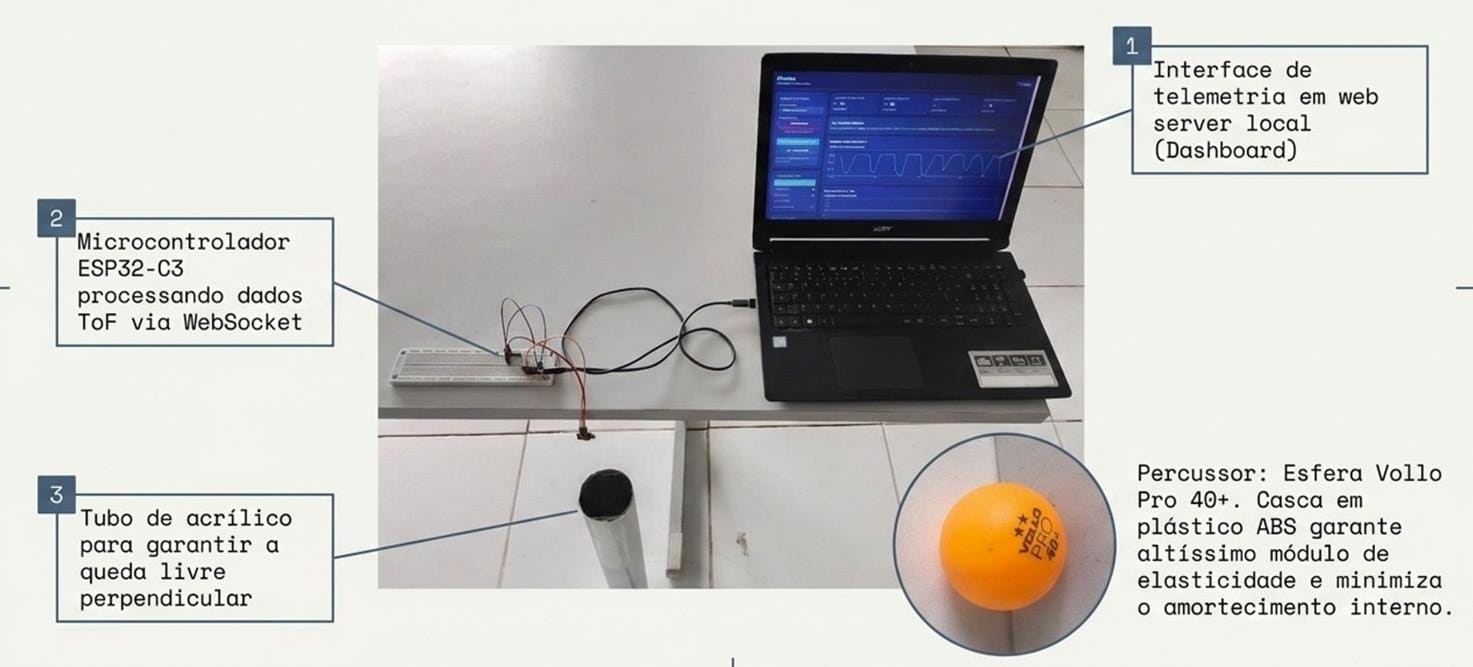
\includegraphics[width=0.75\linewidth]{bancadaDeTeste.jpeg}}
		\caption{Bancada de testes experimental do sistema PisoVibe, evidenciando o tubo de queda vertical e os suportes do conjunto.}
		\label{fig:bancada_teste}
	\end{figure}
	
	O percussor selecionado foi uma esfera polimérica rígida (bola de pingue-pongue Vollo Pro 40+, massa $m \approx 2{,}7$ g, casca fina de plástico ABS), conforme ilustrado na Figura \ref{fig:esfera_percussor}. A escolha técnica do ABS em detrimento de esferas de tênis ou elastômeros macios justifica-se pelo alto módulo de elasticidade e baixíssimo amortecimento interno do material do percussor. Isso garante uma zona de contato extremamente rígida com tempo de colisão infinitesimal, aproximando o impacto a um pulso ideal (Delta de Dirac), o que excita com máxima amplitude as frequências flexurais da laje cerâmica.
	
	\begin{figure}[htbp]
		\centering
		\fbox{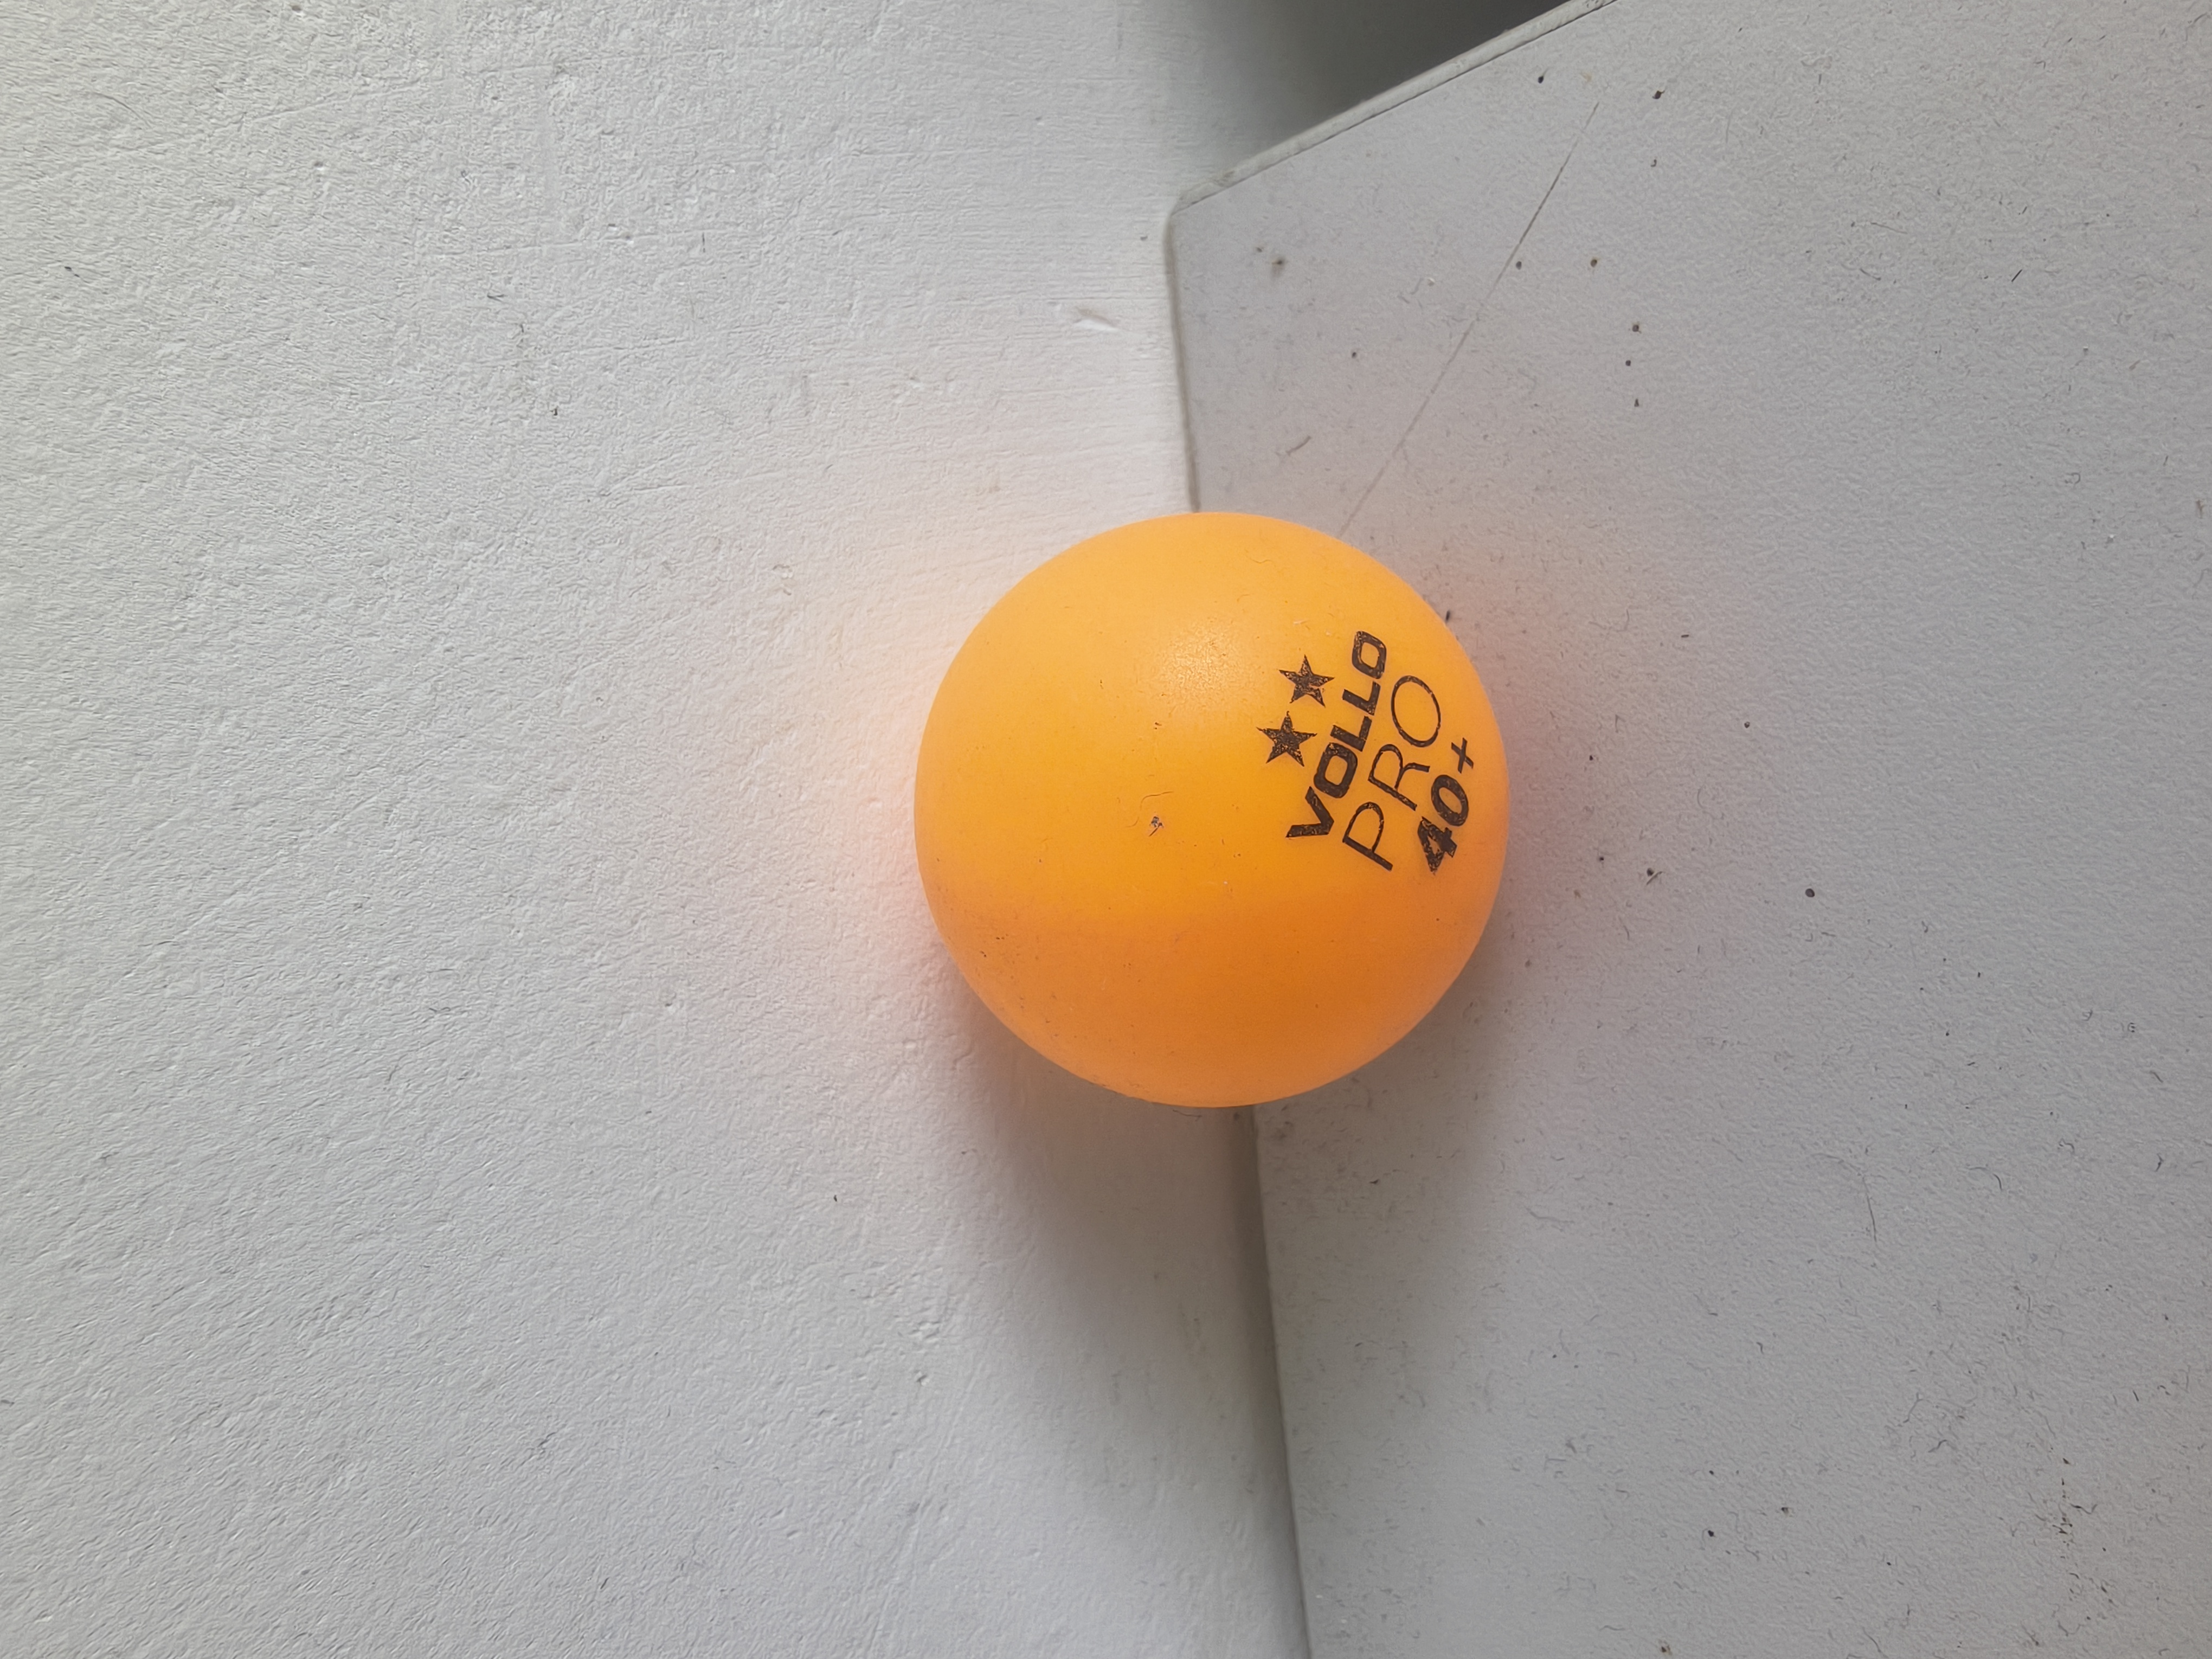
\includegraphics[width=0.7\linewidth]{esfera_percussor.jpg}}
		\caption{Esfera polimérica rígida (Bola de Pingue-Pongue Vollo Pro 40+, $m = 2{,}7\text{ g}$) utilizada para os ensaios de impacto.}
		\label{fig:esfera_percussor}
	\end{figure}
	
	Os ensaios foram realizados em duas condições de contorno de suporte de placas cerâmicas de dimensões idênticas ($30 \times 30$ cm). Podem serem vistas na Figura \ref{fig:corpos_prova}:
	\begin{itemize}[noitemsep]
		\item \textbf{Placa Cerâmica Íntegra (Piso Saudável):} Assentada de maneira uniforme e sólida com argamassa sobre a base de concreto.
		\item \textbf{Placa Cerâmica Fraturada (Piso Ruim):} Apresentando trinca transversal visível e com descolamento parcial induzido de argamassa na subsuperfície.
	\end{itemize}
	
	\begin{figure}[htbp]
		\centering
		\begin{minipage}{0.48\linewidth}
			\centering
			\fbox{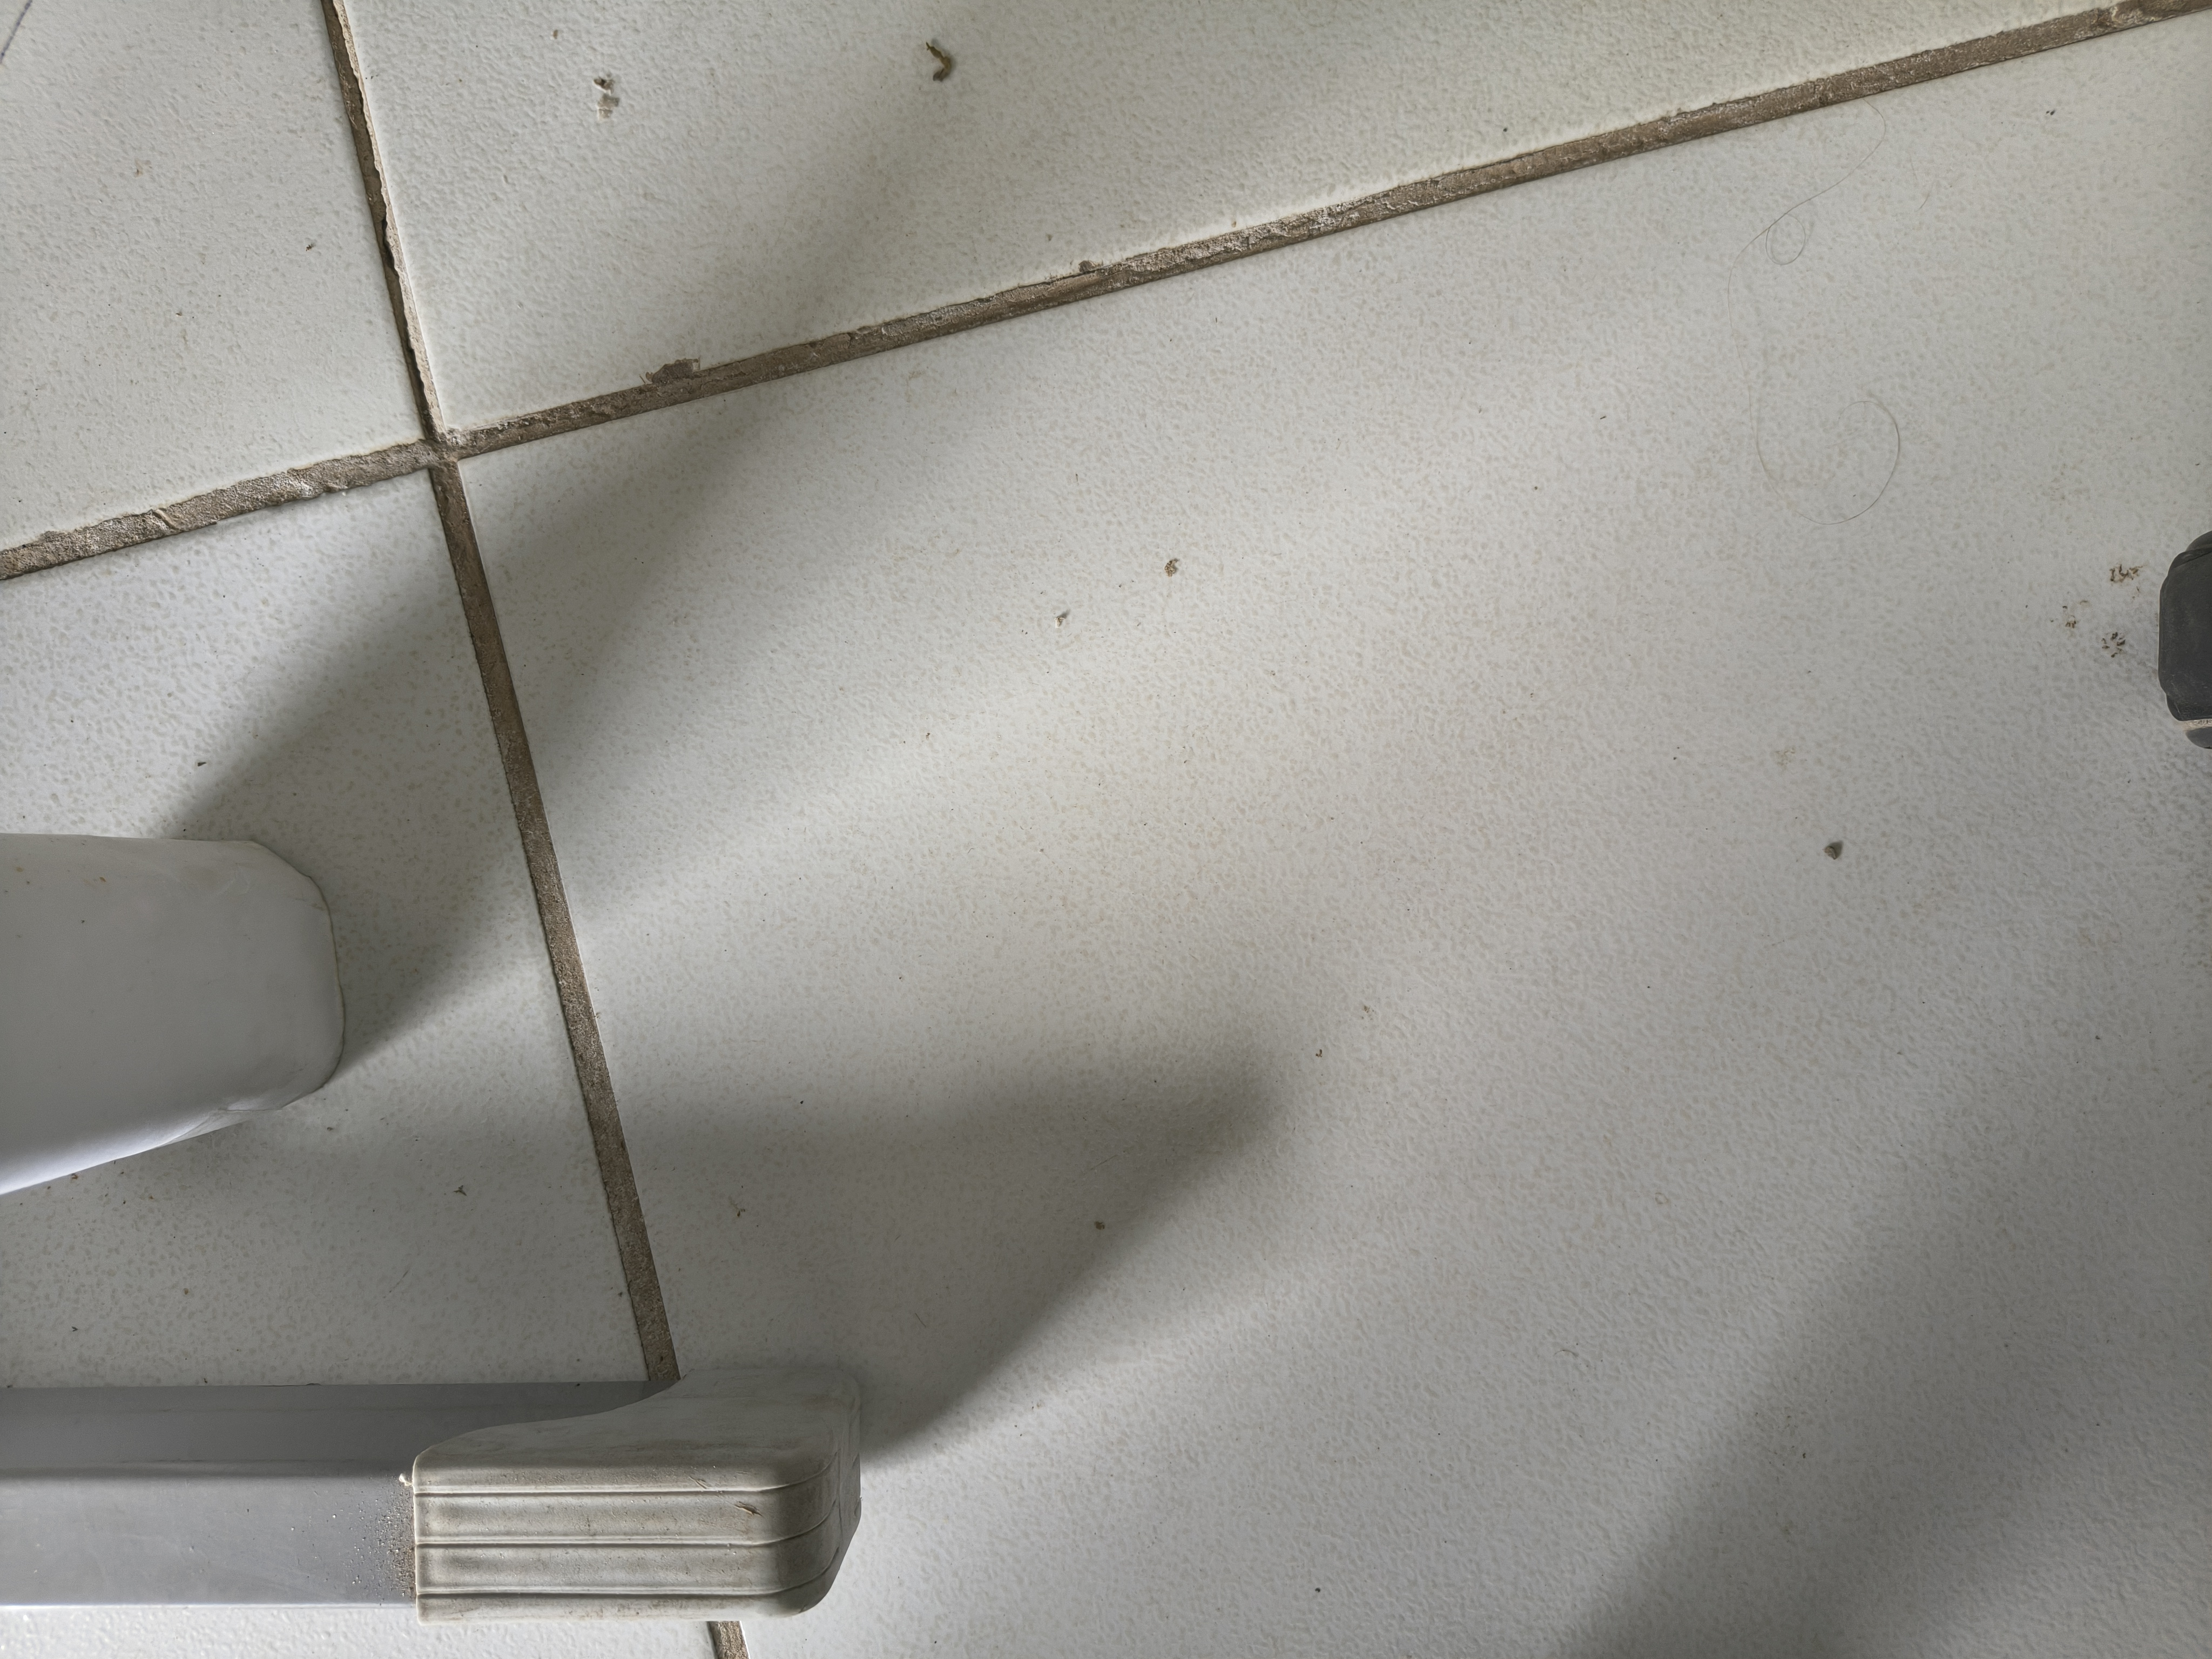
\includegraphics[width=\linewidth]{piso_saudavel.jpg}}
			\caption*{(a) Piso Saudável}
		\end{minipage}
		\hfill
		\begin{minipage}{0.48\linewidth}
			\centering
			\fbox{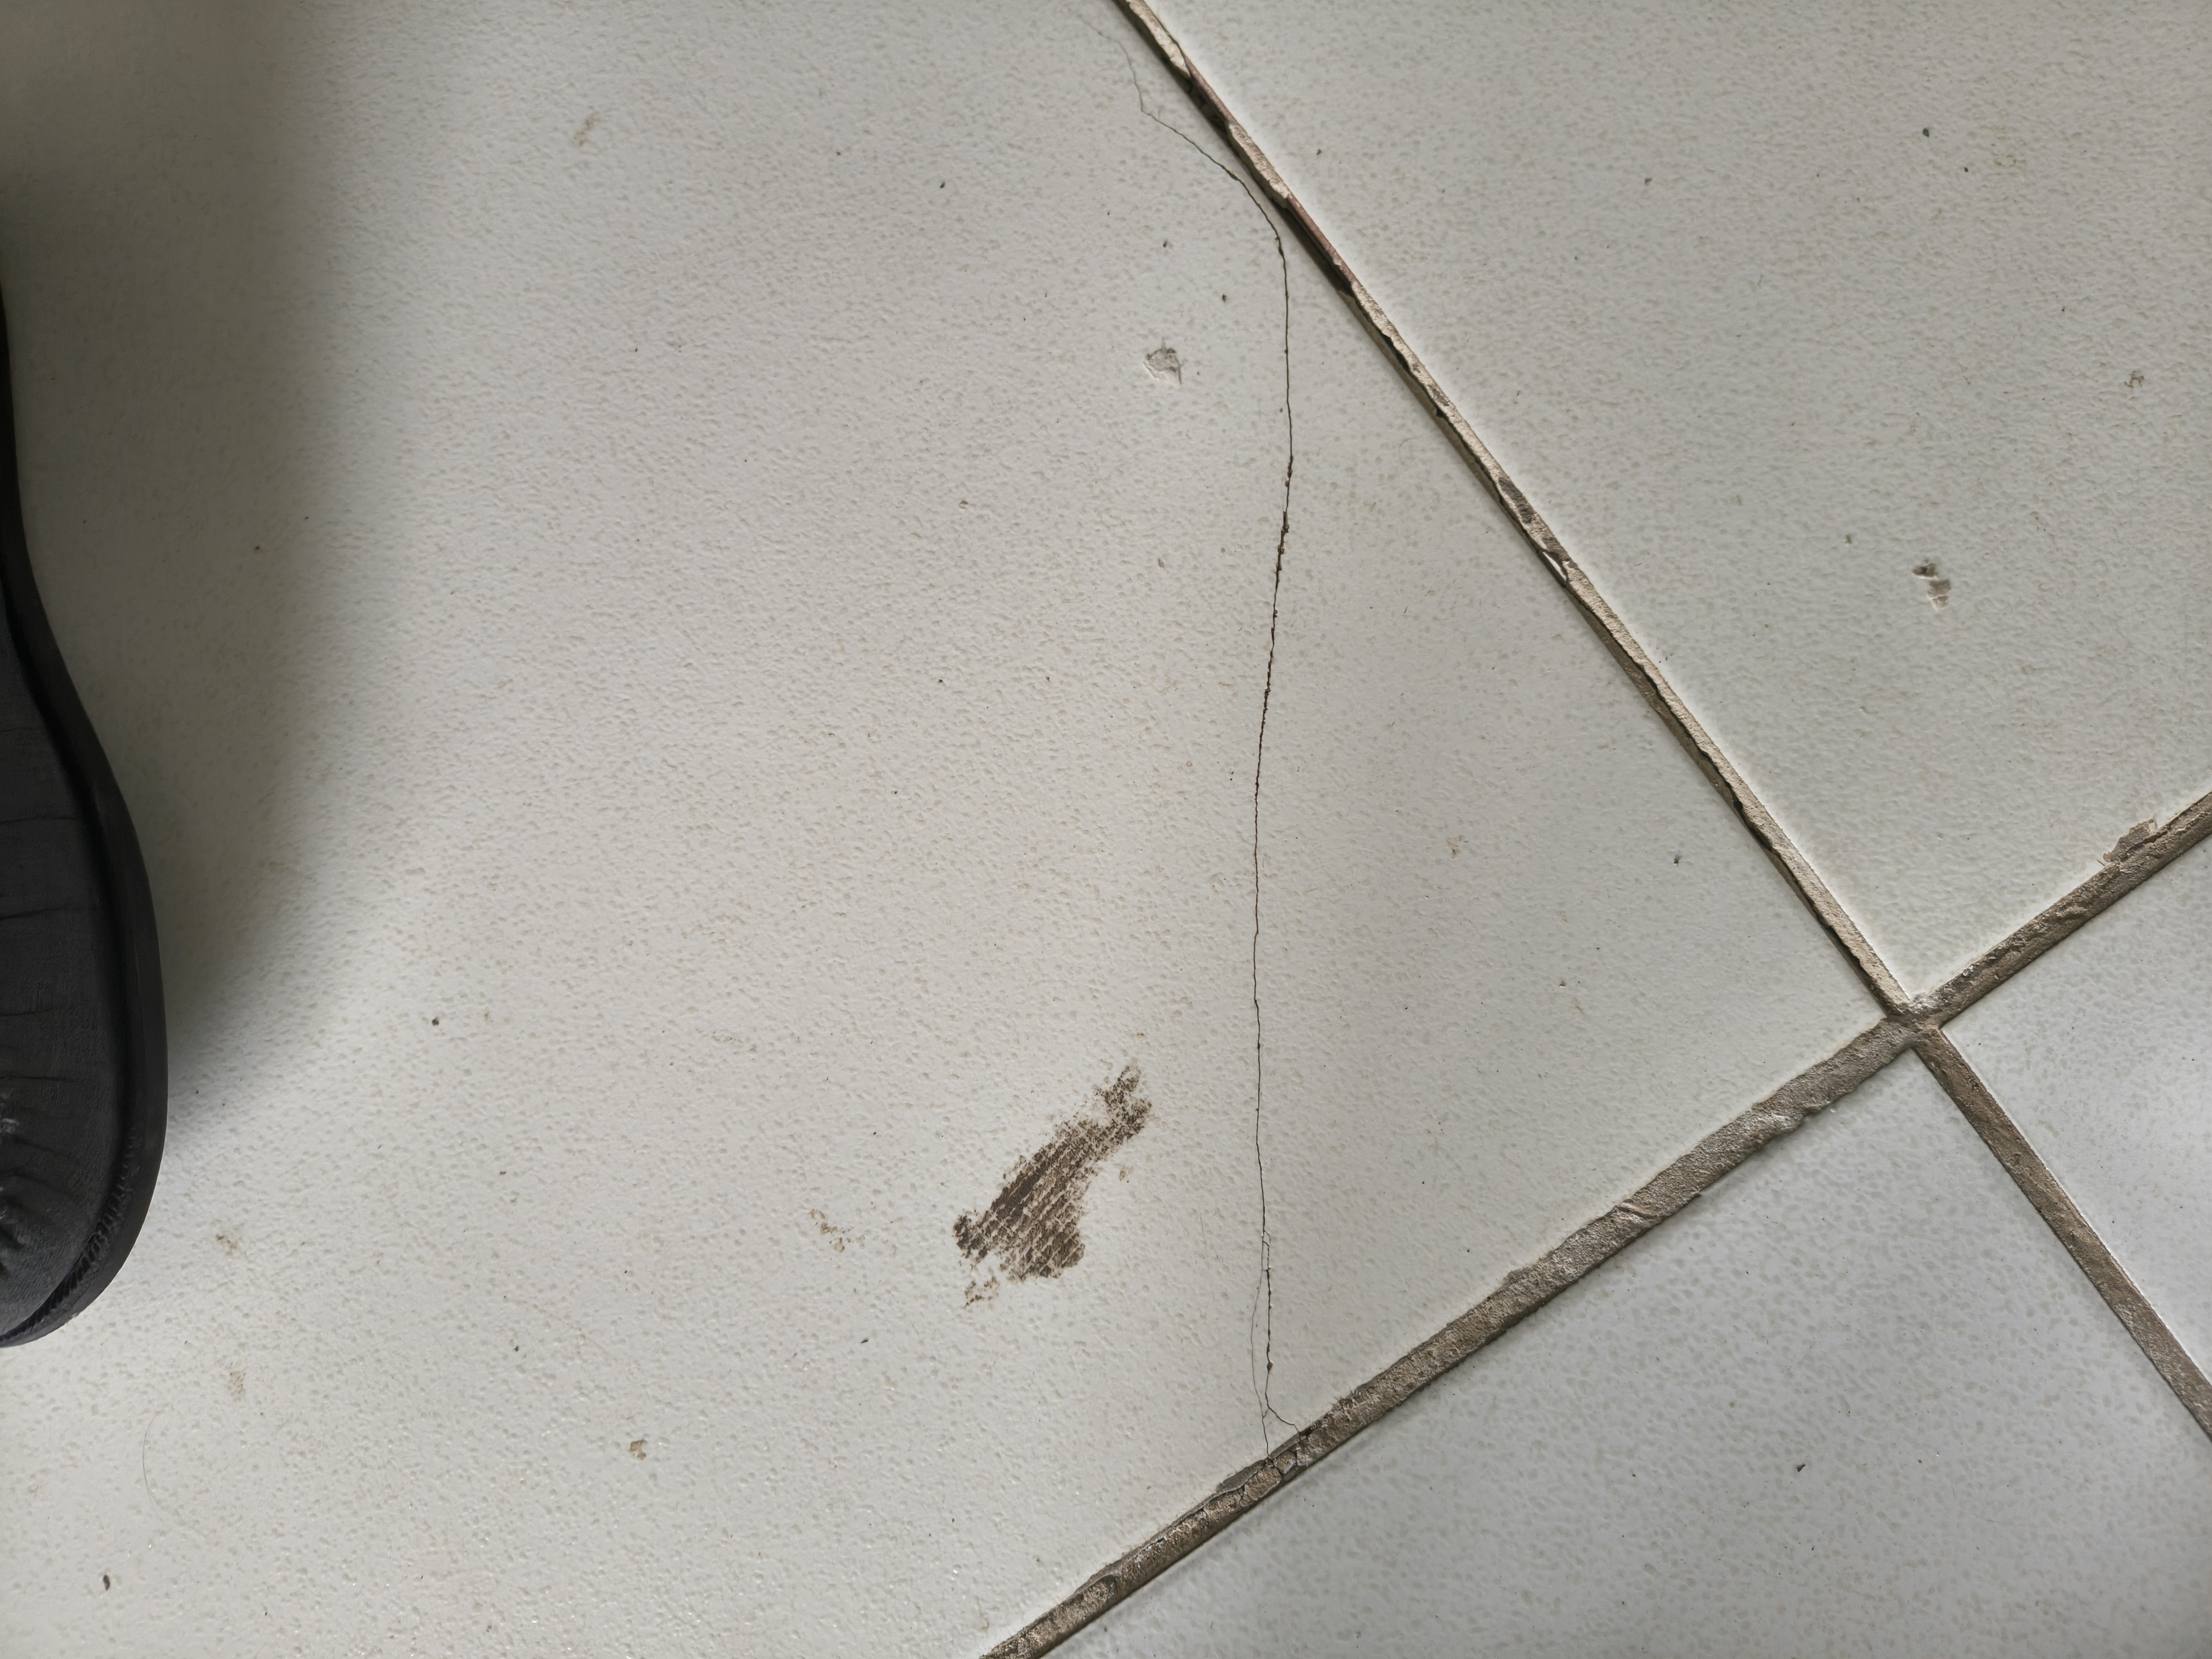
\includegraphics[width=\linewidth]{piso_ruim.jpg}}
			\caption*{(b) Piso Ruim}
		\end{minipage}
		\caption{Condições superficiais dos revestimentos testados: (a) Placa cerâmica íntegra (Piso Saudável); (b) Placa cerâmica fraturada com trinca visível (Piso Ruim).}
		\label{fig:corpos_prova}
	\end{figure}
	
	Os sensores integrados ao sistema foram:
	\begin{itemize}[noitemsep]
		\item \textbf{Sensor Óptico Time-of-Flight (ToF) VL53L0X:} Posicionado no topo do tubo de queda, medindo a distância até a esfera a uma taxa de amostragem de $\approx 33$ Hz.
		\item \textbf{Microfone do Smartphone:} Posicionado na base do tubo de queda livre, captando o transiente sonoro do impacto a uma taxa de amostragem de $48$ kHz no formato PCM de 32 bits flutuantes.
	\end{itemize}
	
	A interface de controle baseou-se em um servidor web embarcado no microcontrolador ESP32-C3 DevKitM-1 (SuperMini), acessado localmente pelo smartphone via rede Wi-Fi. O software utiliza a \textbf{HTML5 Web Audio API} no navegador do celular para iniciar a gravação do áudio síncrono. Ao final da janela configurada de gravação, os dados cinemáticos de altura obtidos pelo ESP32 são enviados via WebSocket e o navegador consolida ambos os vetores no arquivo `pisovibe\_captura.csv`. O processamento numérico subsequente e a extração espectral dos dados consolidados foram realizados em rotinas Python utilizando os algoritmos de processamento de sinais da biblioteca SciPy \parencite{virtanen2020scipy}.
	
	% ============================================================
	% RESULTADOS
	% ============================================================
	\section{Resultados e Discussão}

	O alinhamento temporal entre a trajetória cinemática medida pelo sensor ToF VL53L0X e o sinal acústico revelou sincronismo preciso. Os picos de intensidade de áudio coincidiram exatamente com as coordenadas de deslocamento mínimo (altura $h(t) \to 0$ mm) da esfera de ABS. Como observado no gráfico comparativo da Figura \ref{fig:comparacao_trajetoria}, a trajetória temporal do rebote difere significativamente entre as duas peças cerâmicas. No piso saudável ($h_0 \sim 540$ mm), o primeiro rebote atinge a altura máxima de $h_1 \approx 130$ mm, resultando em um coeficiente de restituição de $e \approx 0{,}49$. O comportamento elástico da colisão é mantido por múltiplos ciclos de quique, resultando em uma trajetória sustentada. Por outro lado, no piso ruim ($h_0 \sim 525$ mm), o primeiro rebote atinge apenas $h_1 \approx 90$ mm, correspondendo a um coeficiente de restituição reduzido de $e \approx 0{,}41$, com decaimento acelerado (quique amortecido).
	
	A perda repentina de altura no piso ruim decorre da deformação da placa na fratura sob o impacto. A abertura transiente da trinca dissipa grande parte da energia mecânica da esfera rígida na forma de atrito interno nas bordas da fratura, impedindo o ricochete eficiente da esfera.
	
	\begin{figure}[htbp]
		\centering
		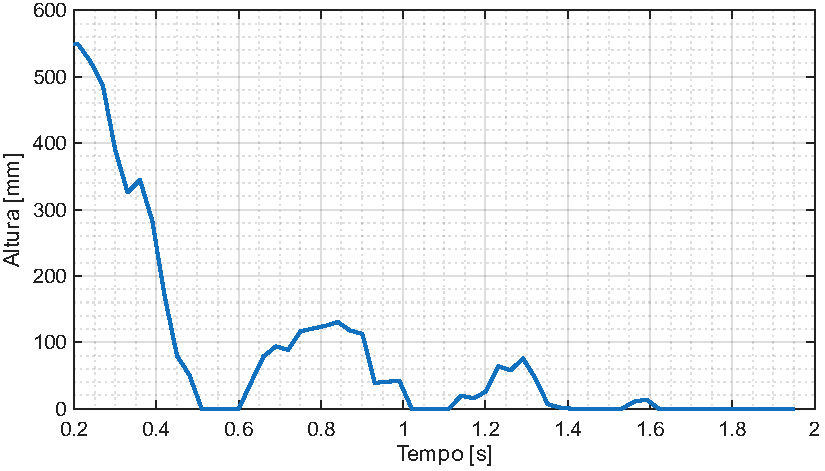
\includegraphics[width=0.98\linewidth]{pisosaudavel.pdf}
		\caption*{(a) Piso Saudável ($e \approx 0{,}49$)}
		\vspace{1.5ex}
		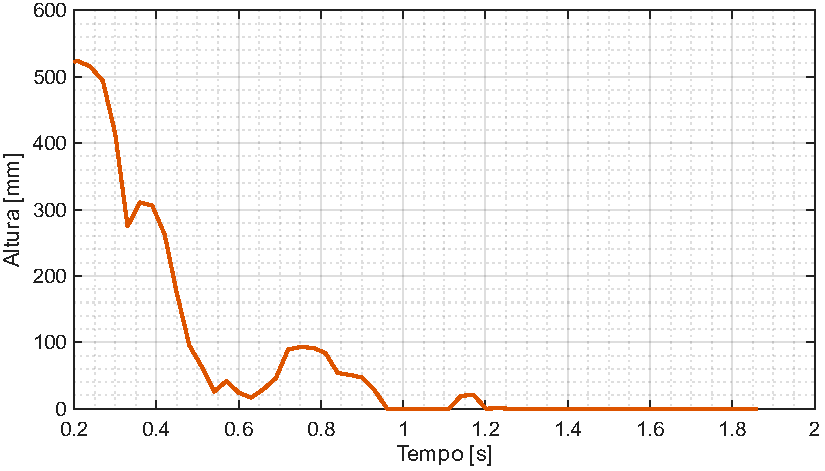
\includegraphics[width=0.98\linewidth]{pisobaguncado.pdf}
		\caption*{(b) Piso Ruim ($e \approx 0{,}41$)}
		\caption{Comparativo da trajetória temporal e altura de rebote da esfera: (a) placa cerâmica íntegra (Piso Saudável, $e \approx 0{,}49$); (b) placa cerâmica fraturada (Piso Ruim, $e \approx 0{,}41$).}
		\label{fig:comparacao_trajetoria}
	\end{figure}

	A resposta acústica transiente gerada no impacto da esfera, como mostra a Figura \ref{fig:comparacao_som}, revela padrões claros de integridade. A pressão sonora radiada do piso saudável mostra um amortecimento suave e uniforme da radiação acústica. 
	
	No piso ruim, o transiente de som exibe picos iniciais mais elevados e uma reverberação complexa com ruído de alta frequência. Este ruído transiente decorre do atrito e contato local entre as bordas fissuradas da cerâmica fraturada sob o pulso de excitação mecânica, gerando um ruído de cisalhamento característico (atrito na trinca).
	
	\begin{figure}[htbp]
		\centering
		\begin{minipage}{0.48\linewidth}
			\centering
			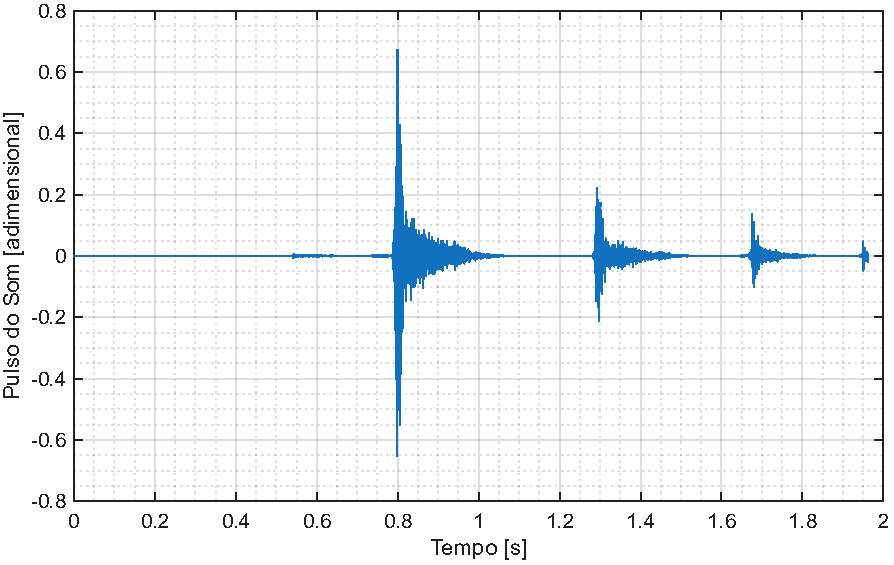
\includegraphics[width=\linewidth]{pulsopisosaudavel.pdf}
			\caption*{(a) Piso Saudável}
		\end{minipage}
		\hfill
		\begin{minipage}{0.48\linewidth}
			\centering
			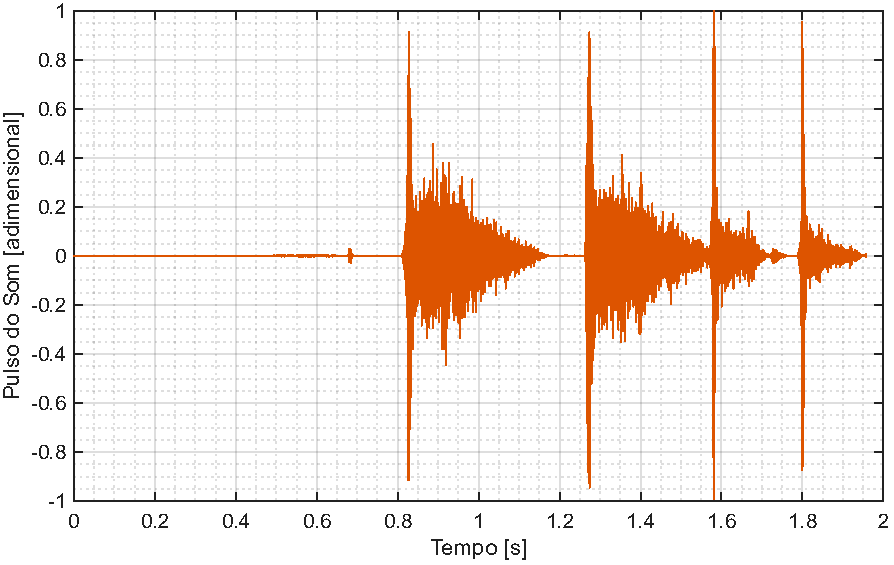
\includegraphics[width=\linewidth]{pulsopisocomdefeito.pdf}
			\caption*{(b) Piso Ruim}
		\end{minipage}
		\caption{Comparação da resposta transiente de pressão sonora gerada no impacto da esfera: (a) placa cerâmica íntegra (Piso Saudável); (b) placa cerâmica fraturada (Piso Ruim).}
		\label{fig:comparacao_som}
	\end{figure}
	
	A análise espectral do impacto sonoro calculada via FFT, conforme mostra a Figura \ref{espectro_fft}, revelou um comportamento físico marcante:
	\begin{itemize}[noitemsep]
		\item No \textbf{Piso Saudável}, a frequência natural dominante é registrada em $f_n = 570{,}0$ Hz, representando o modo flexural de vibração da placa cerâmica perfeitamente engastada sobre o substrato de argamassa colante sólida.
		\item No \textbf{Piso Ruim (Fraturado)}, o pico espectral desloca-se acentuadamente para a alta frequência, registrando uma frequência dominante de **$f_n = 1.880{,}0$ Hz**.
	\end{itemize}
	
	\begin{figure}[htbp]
		\centering
		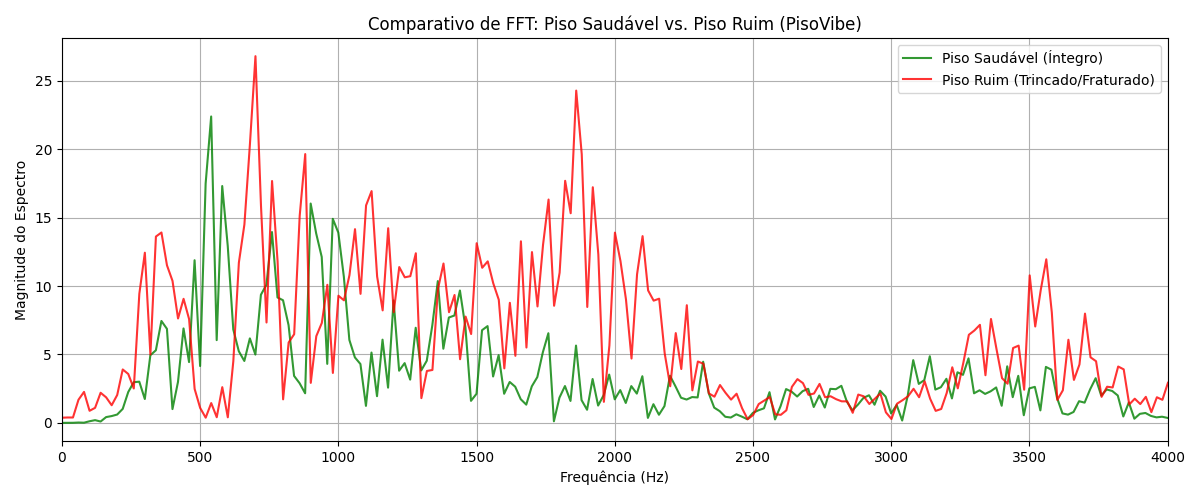
\includegraphics[width=\linewidth]{espectro_fft.png}
		\caption{Espectro de frequência (FFT) do som de impacto: deslocamento da frequência dominante entre a placa íntegra e a placa fraturada.}
		\label{fig:espectro_fft}
	\end{figure}
	
	O deslocamento para alta frequência no piso fraturado contraria a intuição inicial de que a presença de danos diminui a frequência natural devido à redução de rigidez global. No entanto, fisicamente, a trinca transversal visível divide a placa cerâmica de $30 \times 30$ cm em fragmentos independentes menores. 
	
	Como a frequência natural de uma placa está relacionada com a razão rigidez/massa ($\omega_n = \sqrt{k/m}$), a divisão física reduz drasticamente a massa equivalente ($m$) de cada fragmento participante da vibração local sob o ponto de impacto. Como cada pedaço isolado retém uma rigidez relativa elevada, o termo $\sqrt{k/m}$ cresce de forma acentuada, fazendo com que a assinatura acústica ressoe na frequência fundamental muito mais alta de $1.880{,}0$ Hz.
	
	Os dados numéricos finais estão apresentados na Tabela 1 (Piso Saudável) e na Tabela 2 (Piso Fraturado).
	
	O fator de amortecimento acústico ($\zeta$) extraído continuamente via Transformada de Hilbert revelou valores muito semelhantes entre os revestimentos ($\zeta = 1{,}14\%$ no saudável vs. $\zeta = 1{,}20\%$ no fraturado). No entanto, o nível acústico RMS mais elevado no piso fraturado revela a presença de atrito seco e energia radiada na trinca, enquanto o amortecimento mecânico se destaca pela perda total do rebote cinemático.
	
	\begin{table}[!h]
		\centering
		\caption{\textbf{Parâmetros experimentais obtidos para o Piso Saudável (Íntegro).}}
		\label{tab:parametros_saudavel}
		\begin{tabular}{c|c|c}
			\hline
			\textbf{Propriedade} & \textbf{Valor obtido} & \textbf{Comportamento}\\
			\hline
			$h_0$ & 540 & mm \\
			$e$ & $0{,}49$ & adimensional \\
			$f_n$ & $570{,}0$ & Hz \\
			$\zeta$ & $1{,}14$ & \% \\
			RMS & Menor dispersão & dBFS \\
			Rebote & Mantido & Múltiplos quiques \\
			\hline
		\end{tabular}
	\end{table}
	
	\begin{table}[!h]
		\centering
		\caption{\textbf{Parâmetros experimentais obtidos para o Piso Fraturado (Ruim).}}
		\label{tab:parametros_ruim}
		\begin{tabular}{c|c|c}
			\hline
			\textbf{Propriedade} & \textbf{Valor obtido} & \textbf{Diagnóstico / Falha}\\
			\hline
			$h_0$ & 525 & mm \\
			$e$ & $0{,}41$ & Dissipação na trinca \\
			$f_n$ & $1.880{,}0$ & Hz (Alta Frequência) \\
			$\zeta$ & $1{,}20$ & \% \\
			RMS & Picos elevados & Ruído e atrito \\
			Rebote & Amortecido & Perda de energia \\
			\hline
		\end{tabular}
	\end{table}
	
	Não obstante, correlaciona-se diretamente estes resultados técnicas de Engenharia Civil com ensaios não destrutivos (END) normatizados e de larga escala utilizados na engenharia de estruturas, amplamente discutidos na literatura científica para detecção de delaminações e falhas de suporte \parencite{sansalone1997impact, carino2001impact}:
	
	\begin{itemize}[noitemsep]
		\item \textbf{Ensaio de Impact-Echo (ASTM C1383):} Padronizado pela norma técnica internacional \parencite{astmc1383}, utiliza impacto mecânico transiente e processamento de sinal em frequência para detectar delaminações, fissuras internas e avaliar a espessura de placas de concreto. O PisoVibe atua sob o mesmo princípio físico básico da reflexão de ondas de tensão elástica longitudinais (ondas P).
		\item \textbf{Ensaio de Integridade de Estacas (PIT - ASTM D5882):} Normatizado pela \parencite{astmd5882}, onde o topo de uma estaca é percutido com um martelo e a resposta vibracional no tempo é registrada por acelerômetros para mapear variações de impedância acústica ($Z = \rho C A$), onde $\rho$ é a massa específica, $A$ é a seção transversal e $C$ é a velocidade de propagação de onda no meio.
	\end{itemize}
	
	Pela física de propagação de ondas em sólidos, a velocidade $C$ da onda mecânica está relacionada com o Módulo de Elasticidade Dinâmico ($E_d$) do concreto ou argamassa por:
	\begin{equation}
	C = \sqrt{\frac{E_d}{\rho}}
	\end{equation}
	Consequentemente, a variação local de frequência fundamental medida pelo PisoVibe reflete a rigidez local da laje, permitindo estimar variações no módulo de elasticidade dinâmico do substrato de argamassa e traçar correlações empíricas indiretas com a resistência à compressão simples ($f_{ck}$) do contrapiso.
	
	% ============================================================
	% CONCLUSÃO
	% ============================================================
	\section{Conclusões}
	
	A instrumentação proposta permitiu a aquisição milimétrica da cinemática de ricochete da esfera rígida, correlacionando-a com a análise acústica em alta resolução do smartphone, e a análise física integrada indicou que pisos fraturados apresentam rebotes fortemente amortecidos devido à dissipação de energia na fratura, juntamente com um deslocamento da frequência dominante para a faixa de $1.880{,}0$ Hz devido à subdivisão da placa vibrante em fragmentos menores.
	
	Para trabalhos futuros, recomenda-se a validação sistemática dos métodos utilizados em corpos de prova de concreto com falhas de assentamento induzidas de dimensões conhecidas (bolsões de ar e falta de argamassa controlada). Sugere-se também a implementação de algoritmos de Machine Learning (como Máquinas de Vetores de Suporte ou Redes Neurais Artificiais) executados em Python e integrados à interface web para classificar automaticamente a integridade do piso em tempo real na obra.
	
	% ============================================================
	% REFERÊNCIAS BIBLIOGRÁFICAS
	% ============================================================
	\printbibliography[title={Referências}]
	
\end{document}
